\documentclass[a4paper,12pt]{article}
\usepackage{graphicx, geometry, subfigure, amsmath, adjustbox, array}
\geometry{a4paper,left=2cm,right=2cm,top=1cm,bottom=2cm}
\setlength{\baselineskip}{12pt}
\renewcommand\arraystretch{1.5}

\title{Stars and Planets Problem Set \uppercase\expandafter{\romannumeral1}}
\author{Qingru Hu}
\date{\today}

\begin{document}
\maketitle

\section*{\textbf{Exercise \uppercase\expandafter{\romannumeral1}.1 Sun's efficiency}}


\section*{\textbf{Exercise \uppercase\expandafter{\romannumeral1}.2 Color-Magnitude diagram}}
\subsection*{(a)}
I choose the "hipparcos-bright.txt" dataset to draw the 
color-magnitude diagram Fig.\ref{fig1}. The star that has the greatest parallax is 
highlighted with a blue dot and the brightest one with a red dot.
\begin{figure}[htbp]
    \centering
    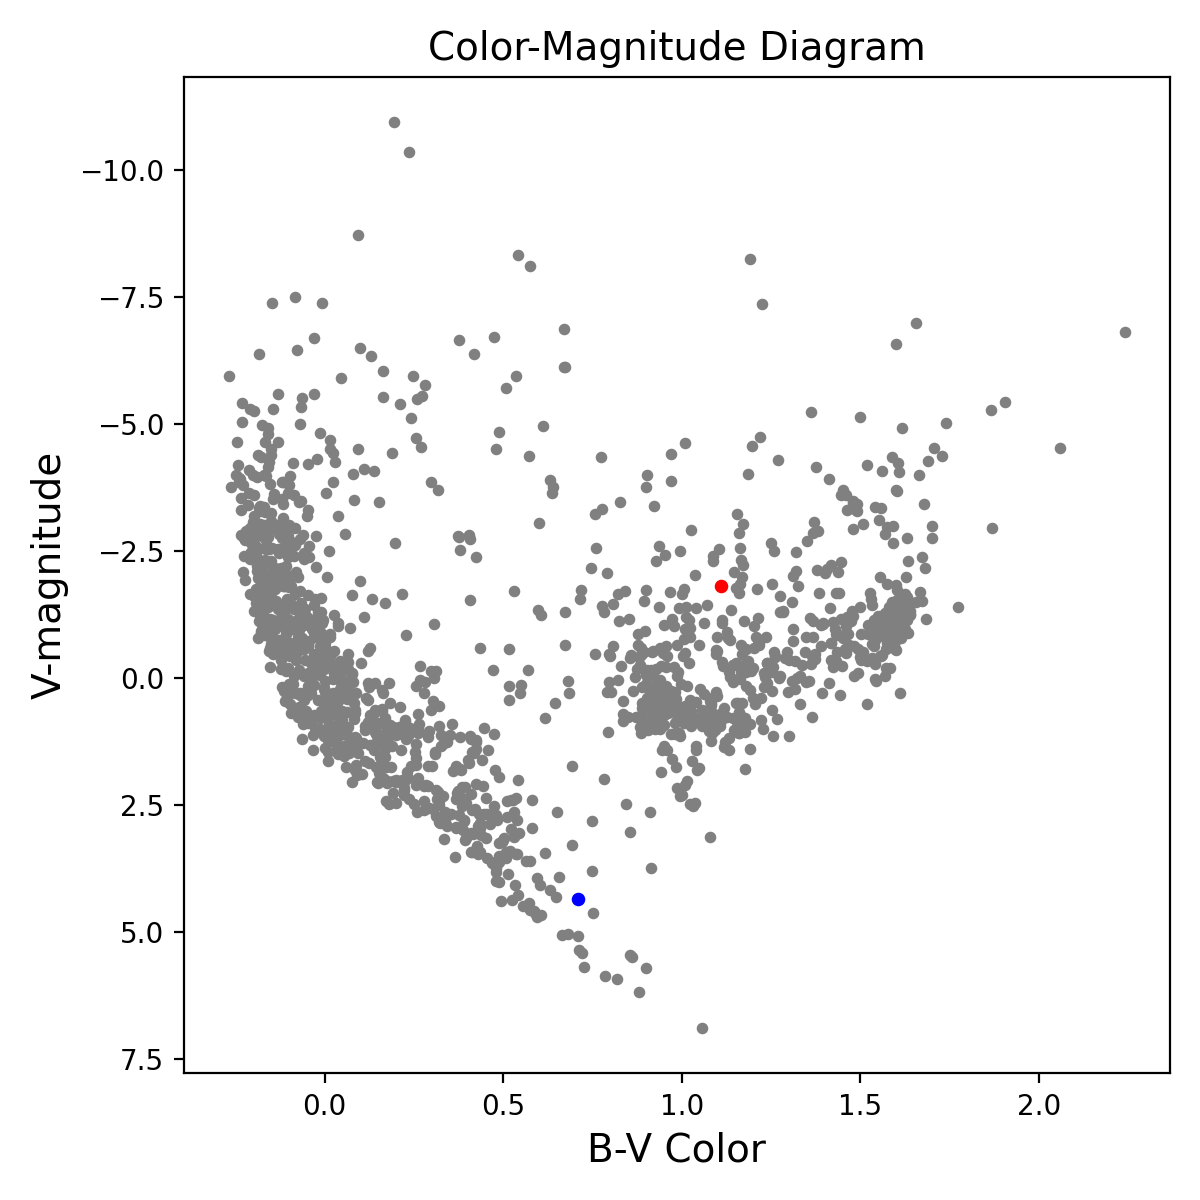
\includegraphics[width=8cm]{color_mag.png}
    \caption{The color-magnitude diagram of "hipparcos-bright.txt"}
    \label{fig1}
\end{figure}

\subsection*{(b)}
That's because for a specific star the apparent and the absolute 
differ only by a constant.
\begin{equation}
    m-M = 5 \text{log}_{10}(\frac{d}{10pc})
\end{equation}
The $B-V$ color index is defined as 
the subtraction of magnitudes at the $B$ and $V$ bands, so the constant 
cancels out.

\subsection*{(c)}
According to the Wien's displacement law:
\begin{equation}
    \lambda_{\text{max}} = \frac{0.2898 \ \text{cm} \ \text{K}}{T}
\end{equation}
the lower the effective temperature $T_{\text{eff}}$, the more radiation 
in the "visual" band (V) and the less radiation in the "blue" band (B). 
Therefore, the star has larger magnitude in the "blue" band (B) 
and smaller magnitude in the "visual" band (V), and their subtraction $B-V$ 
color is higher. That's why stars of higher $B-V$ have lower $T_{\text{eff}}$.

\subsection*{(d)}
The "hipparcos-bright" sample doesn't contain white dwarfs. The main sequence 
stars and the RGB stars are labeled as 
blue and orange respectively in the Fig.\ref{class}. 
I only does a rough classification of these two groups of stars.
\begin{figure}[htbp]
    \centering
    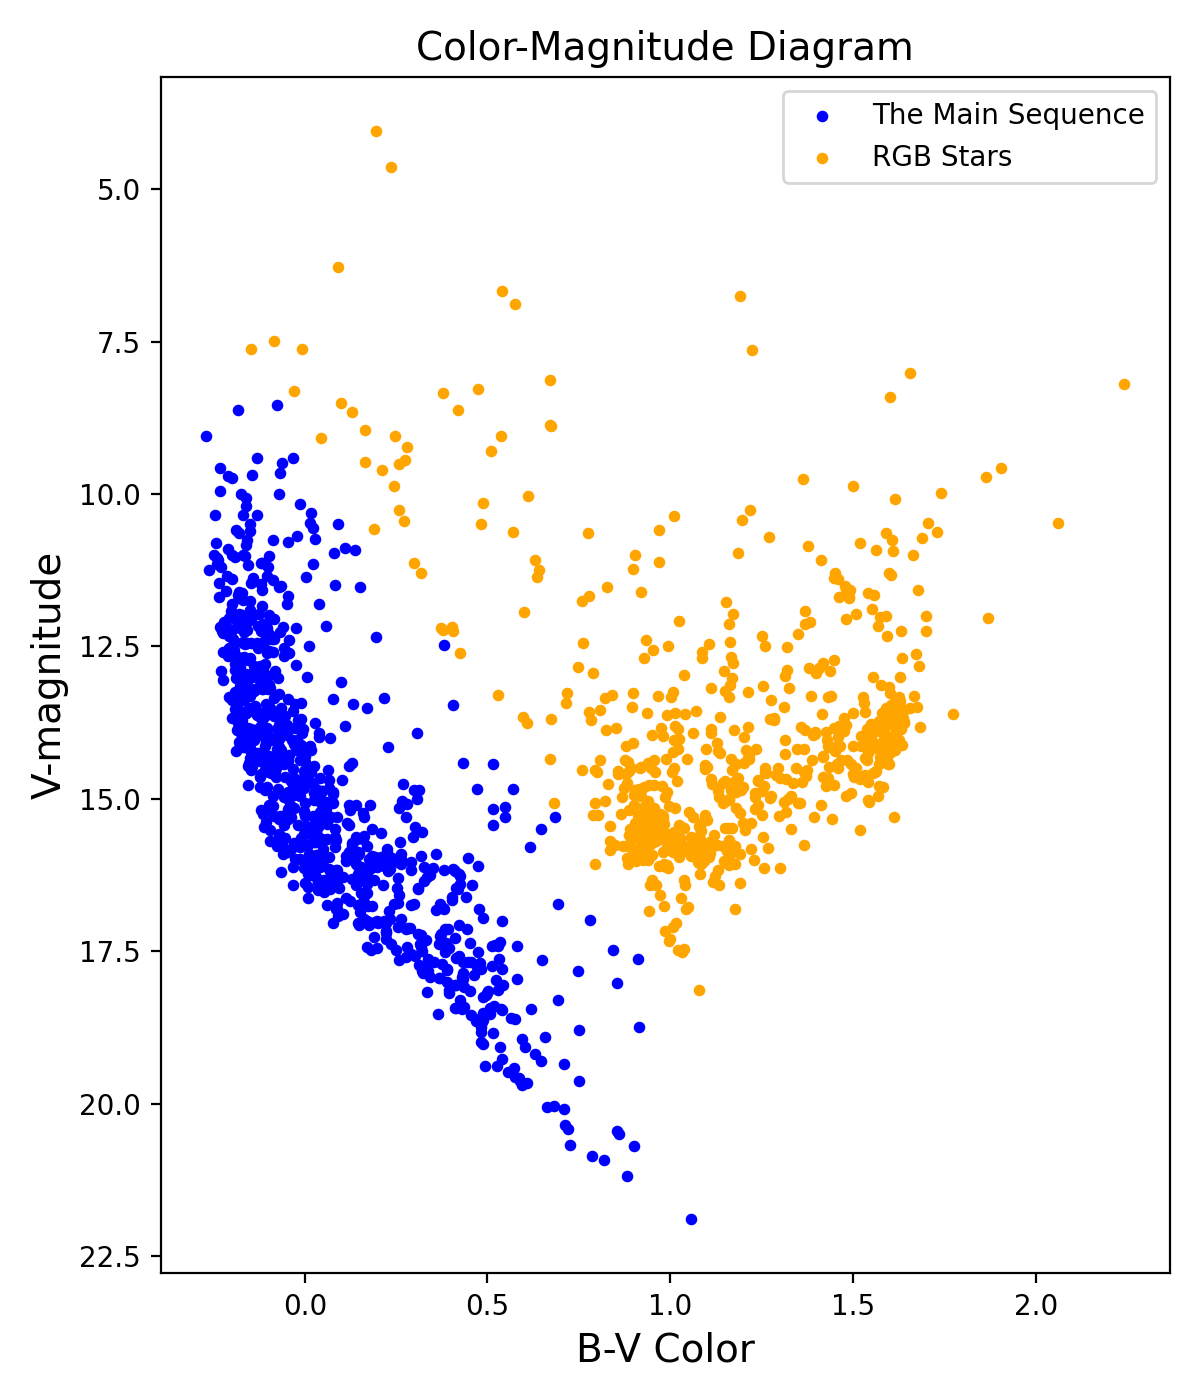
\includegraphics[width=8cm]{two_class.png}
    \caption{The color-magnitude diagram with classification}
    \label{class}
\end{figure}

\subsection*{(e)}


\end{document}
